\section{eo\-Real\-Base\-Vector\-Bounds Class Reference}
\label{classeo_real_base_vector_bounds}\index{eoRealBaseVectorBounds@{eoRealBaseVectorBounds}}
Vector type for bounds (see {\bf eo\-Real\-Bounds.h}{\rm (p.\,\pageref{eo_real_bounds_8h})} for scalar types) ------------ Class {\bf eo\-Real\-Vector\-Bounds}{\rm (p.\,\pageref{classeo_real_vector_bounds})} implements the std::vectorized version: it is basically a std::vector of {\bf eo\-Real\-Bounds}{\rm (p.\,\pageref{classeo_real_bounds})} $\ast$ and forwards all request to the elements of the std::vector.  


{\tt \#include $<$eo\-Real\-Vector\-Bounds.h$>$}

Inheritance diagram for eo\-Real\-Base\-Vector\-Bounds::\begin{figure}[H]
\begin{center}
\leavevmode
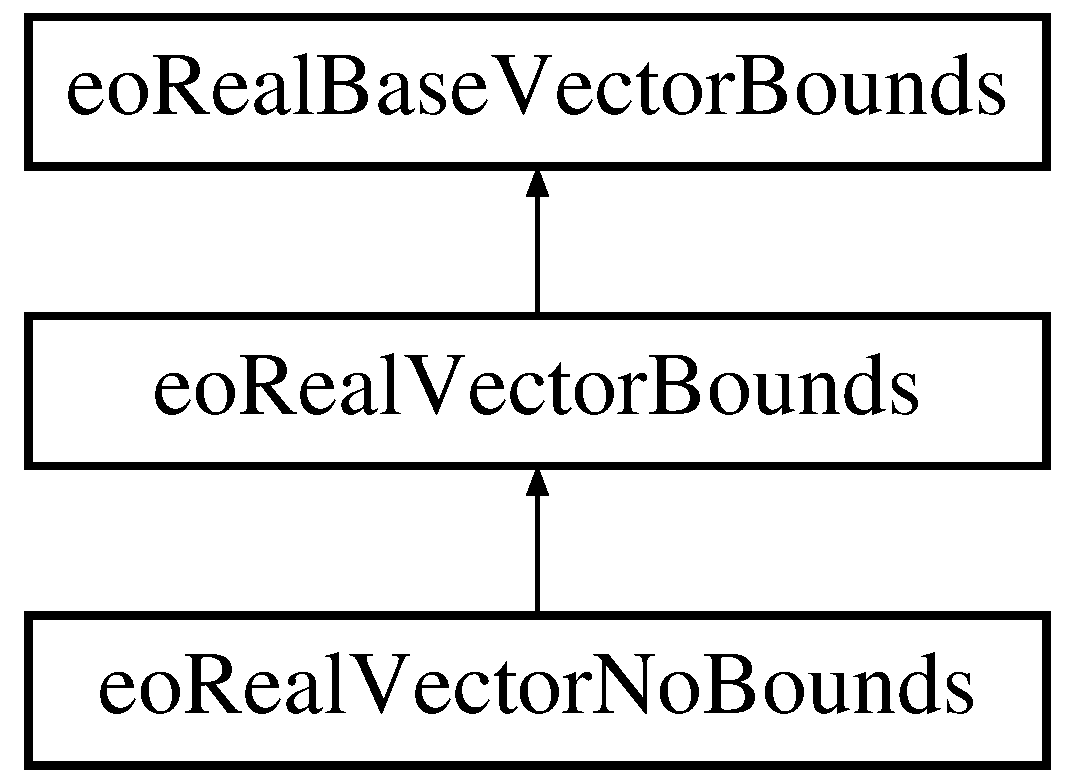
\includegraphics[height=3cm]{classeo_real_base_vector_bounds}
\end{center}
\end{figure}
\subsection*{Public Member Functions}
\begin{CompactItemize}
\item 
{\bf eo\-Real\-Base\-Vector\-Bounds} ()\label{classeo_real_base_vector_bounds_a1}

\begin{CompactList}\small\item\em Default Ctor. \item\end{CompactList}\item 
{\bf eo\-Real\-Base\-Vector\-Bounds} (unsigned \_\-dim, {\bf eo\-Real\-Bounds} \&\_\-bounds)\label{classeo_real_base_vector_bounds_a2}

\begin{CompactList}\small\item\em Ctor: same bounds for everybody, given as an {\bf eo\-Real\-Bounds}{\rm (p.\,\pageref{classeo_real_bounds})}. \item\end{CompactList}\item 
{\bf eo\-Real\-Base\-Vector\-Bounds} ({\bf eo\-Real\-Bounds} \&\_\-xbounds, {\bf eo\-Real\-Bounds} \&\_\-ybounds)\label{classeo_real_base_vector_bounds_a3}

\begin{CompactList}\small\item\em Ctor, particular case of dim-2. \item\end{CompactList}\item 
virtual bool {\bf is\-Bounded} (unsigned \_\-i)\label{classeo_real_base_vector_bounds_a4}

\begin{CompactList}\small\item\em test: is i\_\-th component bounded \item\end{CompactList}\item 
virtual bool {\bf is\-Bounded} (void)\label{classeo_real_base_vector_bounds_a5}

\begin{CompactList}\small\item\em test: bounded iff all are bounded \item\end{CompactList}\item 
virtual bool {\bf has\-No\-Bound\-At\-All} (unsigned \_\-i)\label{classeo_real_base_vector_bounds_a6}

\begin{CompactList}\small\item\em Self-test: true iff i\_\-th component has no bounds at all. \item\end{CompactList}\item 
virtual bool {\bf has\-No\-Bound\-At\-All} (void)\label{classeo_real_base_vector_bounds_a7}

\begin{CompactList}\small\item\em Self-test: true iff all components have no bound at all. \item\end{CompactList}\item 
virtual bool {\bf is\-Min\-Bounded} (unsigned \_\-i)\label{classeo_real_base_vector_bounds_a8}

\item 
virtual bool {\bf is\-Max\-Bounded} (unsigned \_\-i)\label{classeo_real_base_vector_bounds_a9}

\item 
virtual void {\bf folds\-In\-Bounds} (unsigned \_\-i, double \&\_\-r)\label{classeo_real_base_vector_bounds_a10}

\begin{CompactList}\small\item\em Folds a real value back into the bounds - i\_\-th component. \item\end{CompactList}\item 
virtual void {\bf folds\-In\-Bounds} (std::vector$<$ double $>$ \&\_\-v)\label{classeo_real_base_vector_bounds_a11}

\begin{CompactList}\small\item\em Folds all variables of a std::vector of real values into the bounds. \item\end{CompactList}\item 
virtual void {\bf truncate} (unsigned \_\-i, double \&\_\-r)\label{classeo_real_base_vector_bounds_a12}

\begin{CompactList}\small\item\em Truncates a real value to the bounds - i\_\-th component. \item\end{CompactList}\item 
virtual void {\bf truncate} (std::vector$<$ double $>$ \&\_\-v)\label{classeo_real_base_vector_bounds_a13}

\begin{CompactList}\small\item\em truncates all variables of a std::vector of real values to the bounds \item\end{CompactList}\item 
virtual bool {\bf is\-In\-Bounds} (unsigned \_\-i, double \_\-r)\label{classeo_real_base_vector_bounds_a14}

\begin{CompactList}\small\item\em test: is i\_\-th component within the bounds? \item\end{CompactList}\item 
virtual bool {\bf is\-In\-Bounds} (std::vector$<$ double $>$ \_\-v)\label{classeo_real_base_vector_bounds_a15}

\begin{CompactList}\small\item\em test: are ALL components within the bounds? \item\end{CompactList}\item 
virtual double {\bf minimum} (unsigned \_\-i)\label{classeo_real_base_vector_bounds_a16}

\begin{CompactList}\small\item\em Accessors: will raise an std::exception if these do not exist. \item\end{CompactList}\item 
virtual double {\bf maximum} (unsigned \_\-i)\label{classeo_real_base_vector_bounds_a17}

\item 
virtual double {\bf range} (unsigned \_\-i)\label{classeo_real_base_vector_bounds_a18}

\item 
virtual double {\bf average\-Range} ()\label{classeo_real_base_vector_bounds_a19}

\begin{CompactList}\small\item\em Computes the average range An std::exception will be raised if one of the component is unbounded. \item\end{CompactList}\item 
virtual double {\bf uniform} (unsigned \_\-i, {\bf eo\-Rng} \&\_\-rng=eo::rng)\label{classeo_real_base_vector_bounds_a20}

\begin{CompactList}\small\item\em Generates a random number in i\_\-th range An std::exception will be raised if one of the component is unbounded. \item\end{CompactList}\item 
void {\bf uniform} (std::vector$<$ double $>$ \&\_\-v, {\bf eo\-Rng} \&\_\-rng=eo::rng)\label{classeo_real_base_vector_bounds_a21}

\begin{CompactList}\small\item\em fills a std::vector with uniformly chosen variables in bounds An std::exception will be raised if one of the component is unbounded \item\end{CompactList}\item 
virtual void {\bf print\-On} (std::ostream \&\_\-os) const 
\begin{CompactList}\small\item\em Write object. \item\end{CompactList}\end{CompactItemize}


\subsection{Detailed Description}
Vector type for bounds (see {\bf eo\-Real\-Bounds.h}{\rm (p.\,\pageref{eo_real_bounds_8h})} for scalar types) ------------ Class {\bf eo\-Real\-Vector\-Bounds}{\rm (p.\,\pageref{classeo_real_vector_bounds})} implements the std::vectorized version: it is basically a std::vector of {\bf eo\-Real\-Bounds}{\rm (p.\,\pageref{classeo_real_bounds})} $\ast$ and forwards all request to the elements of the std::vector. 

This file also contains the global variables and eo\-Dummy\-Vector\-No\-Bounds that are used as defaults in ctors (i.e. when no bounds are given, it is assumed unbounded values)

THe 2 main classes defined here are

eo\-Real\-Base\-Vector\-Bounds, base class that handles all useful functions {\bf eo\-Real\-Vector\-Bounds}{\rm (p.\,\pageref{classeo_real_vector_bounds})} which derives from the preceding $\ast$and$\ast$ {\bf eo\-Persistent}{\rm (p.\,\pageref{classeo_persistent})} and also has a mechanism for memory handling of the pointers it has to allocate 



Definition at line 58 of file eo\-Real\-Vector\-Bounds.h.

\subsection{Member Function Documentation}
\index{eoRealBaseVectorBounds@{eo\-Real\-Base\-Vector\-Bounds}!printOn@{printOn}}
\index{printOn@{printOn}!eoRealBaseVectorBounds@{eo\-Real\-Base\-Vector\-Bounds}}
\subsubsection{\setlength{\rightskip}{0pt plus 5cm}virtual void eo\-Real\-Base\-Vector\-Bounds::print\-On (std::ostream \& {\em \_\-os}) const\hspace{0.3cm}{\tt  [inline, virtual]}}\label{classeo_real_base_vector_bounds_a22}


Write object. 

It's called print\-On since it prints the object on a stream. \begin{Desc}
\item[Parameters:]
\begin{description}
\item[{\em \_\-os}]A std::ostream. \end{description}
\end{Desc}


Reimplemented in {\bf eo\-Real\-Vector\-Bounds} {\rm (p.\,\pageref{classeo_real_vector_bounds_a9})}.

Definition at line 214 of file eo\-Real\-Vector\-Bounds.h.

The documentation for this class was generated from the following file:\begin{CompactItemize}
\item 
eo\-Real\-Vector\-Bounds.h\end{CompactItemize}
